\documentclass{article}
%\usepackage{../public/pgf-umlcd-f}
\usepackage{pgf-umlcd}
%xeCJK
\usepackage[BoldFont,SlantFont,CJKchecksingle]{xeCJK}
\setCJKmainfont[BoldFont=SimHei,SlantedFont=KaiTi]{SimSun}

\begin{document}
\section{Common Layer}
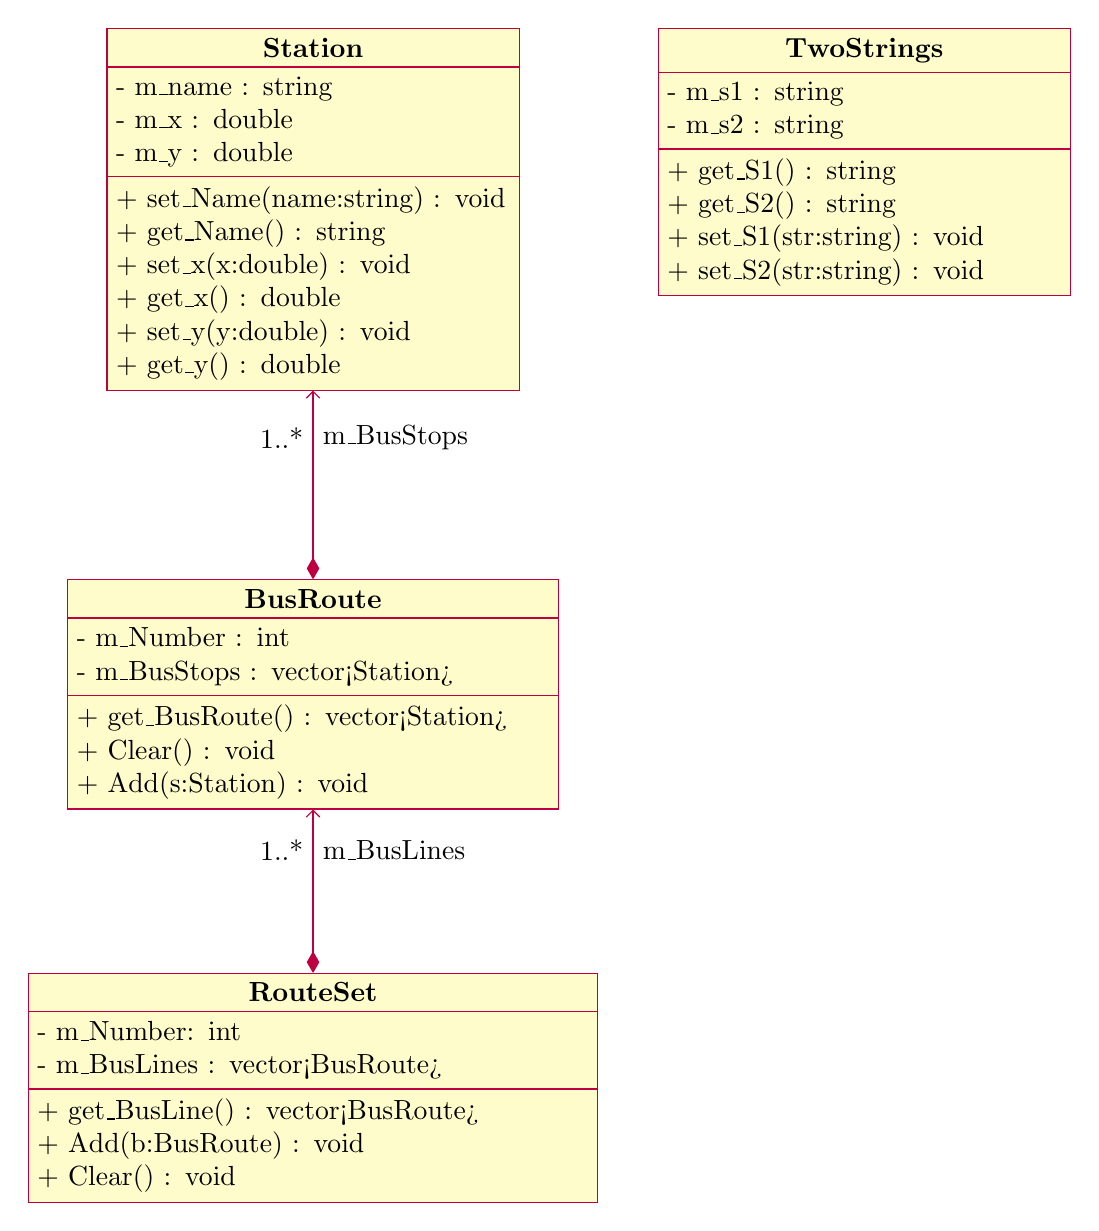
\begin{tikzpicture}
\begin{class}{Station}{0,0}
\attribute{- m\_name : string}
\attribute{- m\_x : double}
\attribute{- m\_y : double}
\operation{+ set\_Name(name:string) : void}
\operation{+ get\_Name() : string}
\operation{+ set\_x(x:double) : void}
\operation{+ get\_x() : double}
\operation{+ set\_y(y:double) : void}
\operation{+ get\_y() : double}
\end{class}
\begin{class}[text width=6cm]{BusRoute}{0,-7}
\attribute{- m\_Number : int}
\attribute{- m\_BusStops : vector<Station>}
\operation{+ get\_BusRoute() : vector<Station>}
\operation{+ Clear() : void}
\operation{+ Add(s:Station) : void}
\end{class}
\begin{class}[text width=7cm]{RouteSet}{0,-12}
\attribute{- m\_Number: int}
\attribute{- m\_BusLines : vector<BusRoute>}
\operation{+ get\_BusLine() : vector<BusRoute>}
\operation{+ Add(b:BusRoute) : void}
\operation{+ Clear() : void}
\end{class}
\composition{BusRoute}{1..*}{m\_BusStops}{Station}
\composition{RouteSet}{1..*}{m\_BusLines}{BusRoute}
\begin{class}{TwoStrings}{7,0}
\attribute{- m\_s1 : string}
\attribute{- m\_s2 : string}
\operation{+ get\_S1() : string}
\operation{+ get\_S2() : string}
\operation{+ set\_S1(str:string) : void}
\operation{+ set\_S2(str:string) : void}
\end{class}
\end{tikzpicture}
\newpage

\section{Model Layer}
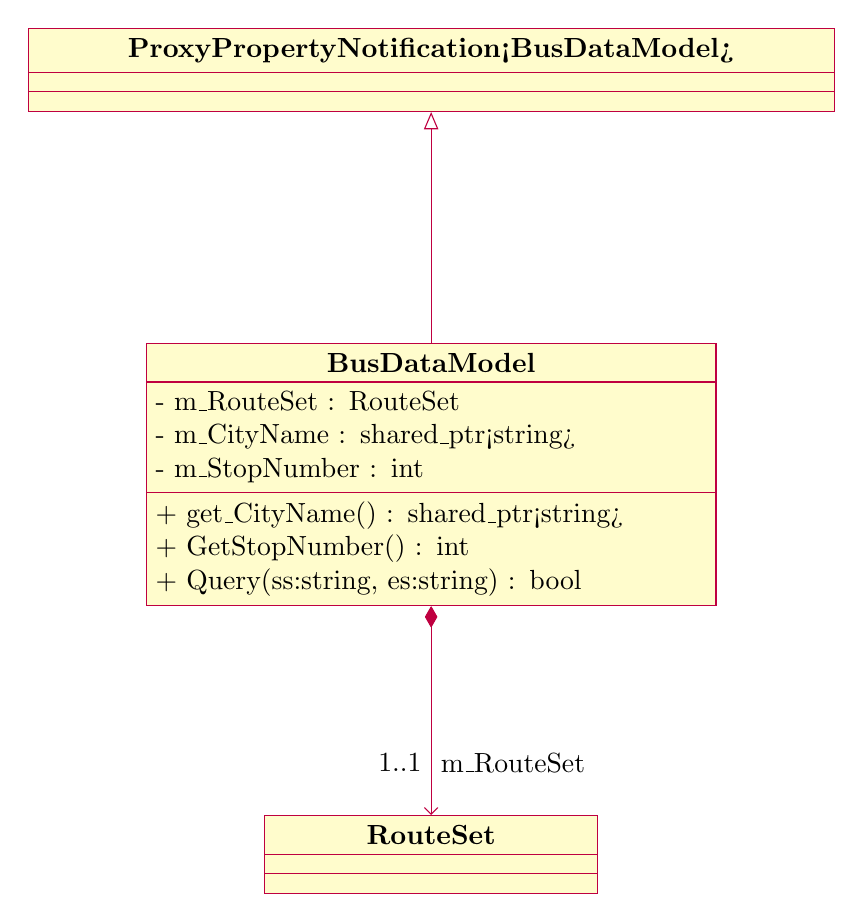
\begin{tikzpicture}
\begin{class}[text width=4cm]{RouteSet}{0,-10}\end{class}
\begin{class}[text width=10cm]{ProxyPropertyNotification<BusDataModel>}{0,0}\end{class}
\begin{class}[text width=7cm]{BusDataModel}{0,-4}
\inherit{ProxyPropertyNotification<BusDataModel>}
\attribute{- m\_RouteSet : RouteSet}
\attribute{- m\_CityName : shared\_ptr<string>}
\attribute{- m\_StopNumber : int}
\operation{+ get\_CityName() : shared\_ptr<string>}
\operation{+ GetStopNumber() : int}
\operation{+ Query(ss:string, es:string) : bool}
\end{class}
\composition{BusDataModel}{m\_RouteSet}{1..1}{RouteSet}
\end{tikzpicture}
\newpage

\section{ViewModel Layer}
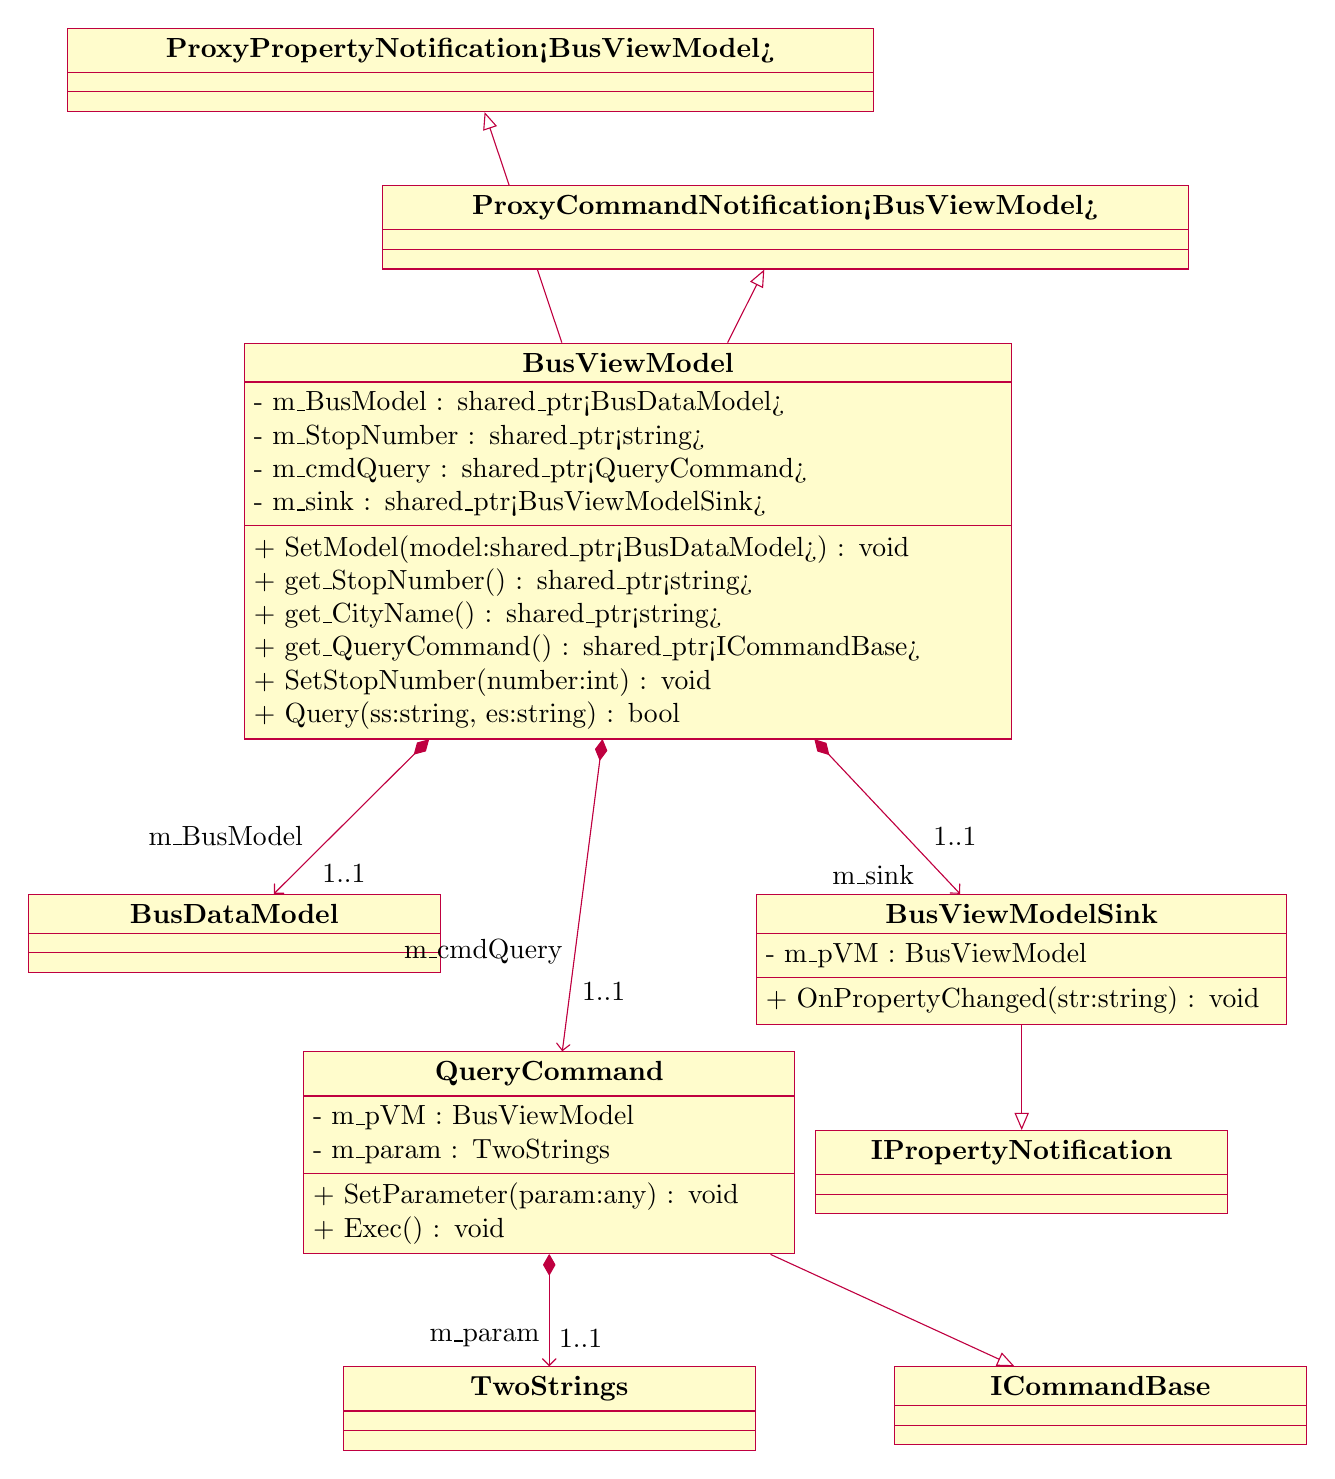
\begin{tikzpicture}
\begin{class}[text width=10cm]{ProxyPropertyNotification<BusViewModel>}{-3,0}\end{class}
\begin{class}[text width=10cm]{ProxyCommandNotification<BusViewModel>}{1,-2}\end{class}
\begin{class}{BusDataModel}{-6,-11}\end{class}
\begin{class}[text width=9.5cm]{BusViewModel}{-1,-4}
\inherit{ProxyPropertyNotification<BusViewModel>}
\inherit{ProxyCommandNotification<BusViewModel>}
\attribute{- m\_BusModel : shared\_ptr<BusDataModel>}
\attribute{- m\_StopNumber : shared\_ptr<string>}
\attribute{- m\_cmdQuery : shared\_ptr<QueryCommand>}
\attribute{- m\_sink : shared\_ptr<BusViewModelSink>}
\operation{+ SetModel(model:shared\_ptr<BusDataModel>) : void}
\operation{+ get\_StopNumber() : shared\_ptr<string>}
\operation{+ get\_CityName() : shared\_ptr<string>}
\operation{+ get\_QueryCommand() : shared\_ptr<ICommandBase>}
\operation{+ SetStopNumber(number:int) : void}
\operation{+ Query(ss:string, es:string) : bool}
\end{class}
\begin{class}{ICommandBase}{5,-17}\end{class}
\begin{class}{TwoStrings}{-2,-17}\end{class}
\begin{class}[text width=6cm]{QueryCommand}{-2,-13}
\inherit{ICommandBase}
\attribute{- m\_pVM : BusViewModel}
\attribute{- m\_param : TwoStrings}
\operation{+ SetParameter(param:any) : void}
\operation{+ Exec() : void}
\end{class}
\begin{class}{IPropertyNotification}{4,-14}\end{class}
\begin{class}[text width=6.5cm]{BusViewModelSink}{4,-11}
\inherit{IPropertyNotification}
\attribute{- m\_pVM : BusViewModel}
\operation{+ OnPropertyChanged(str:string) : void}
\end{class}
\composition{BusViewModel}{1..1}{m\_cmdQuery}{QueryCommand}
\composition{BusViewModel}{1..1}{m\_sink}{BusViewModelSink}
\composition{BusViewModel}{1..1}{m\_BusModel}{BusDataModel}
\composition{QueryCommand}{1..1}{m\_param}{TwoStrings}
\end{tikzpicture}
\newpage

\section{View Layer}
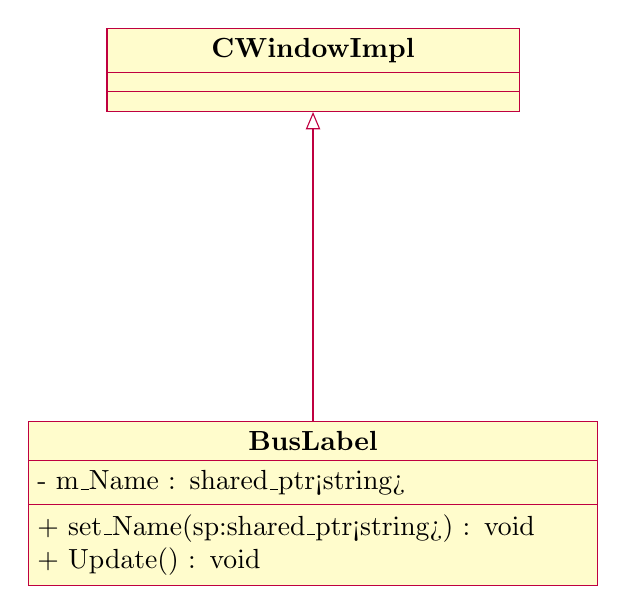
\begin{tikzpicture}
\begin{class}{CWindowImpl}{0,0}
\end{class}
\begin{class}[text width=7cm]{BusLabel}{0,-5}
\inherit{CWindowImpl}
\attribute{- m\_Name : shared\_ptr<string>}
\operation{+ set\_Name(sp:shared\_ptr<string>) : void}
\operation{+ Update() : void}
\end{class}
\end{tikzpicture}
\newpage

\section{Window Layer}
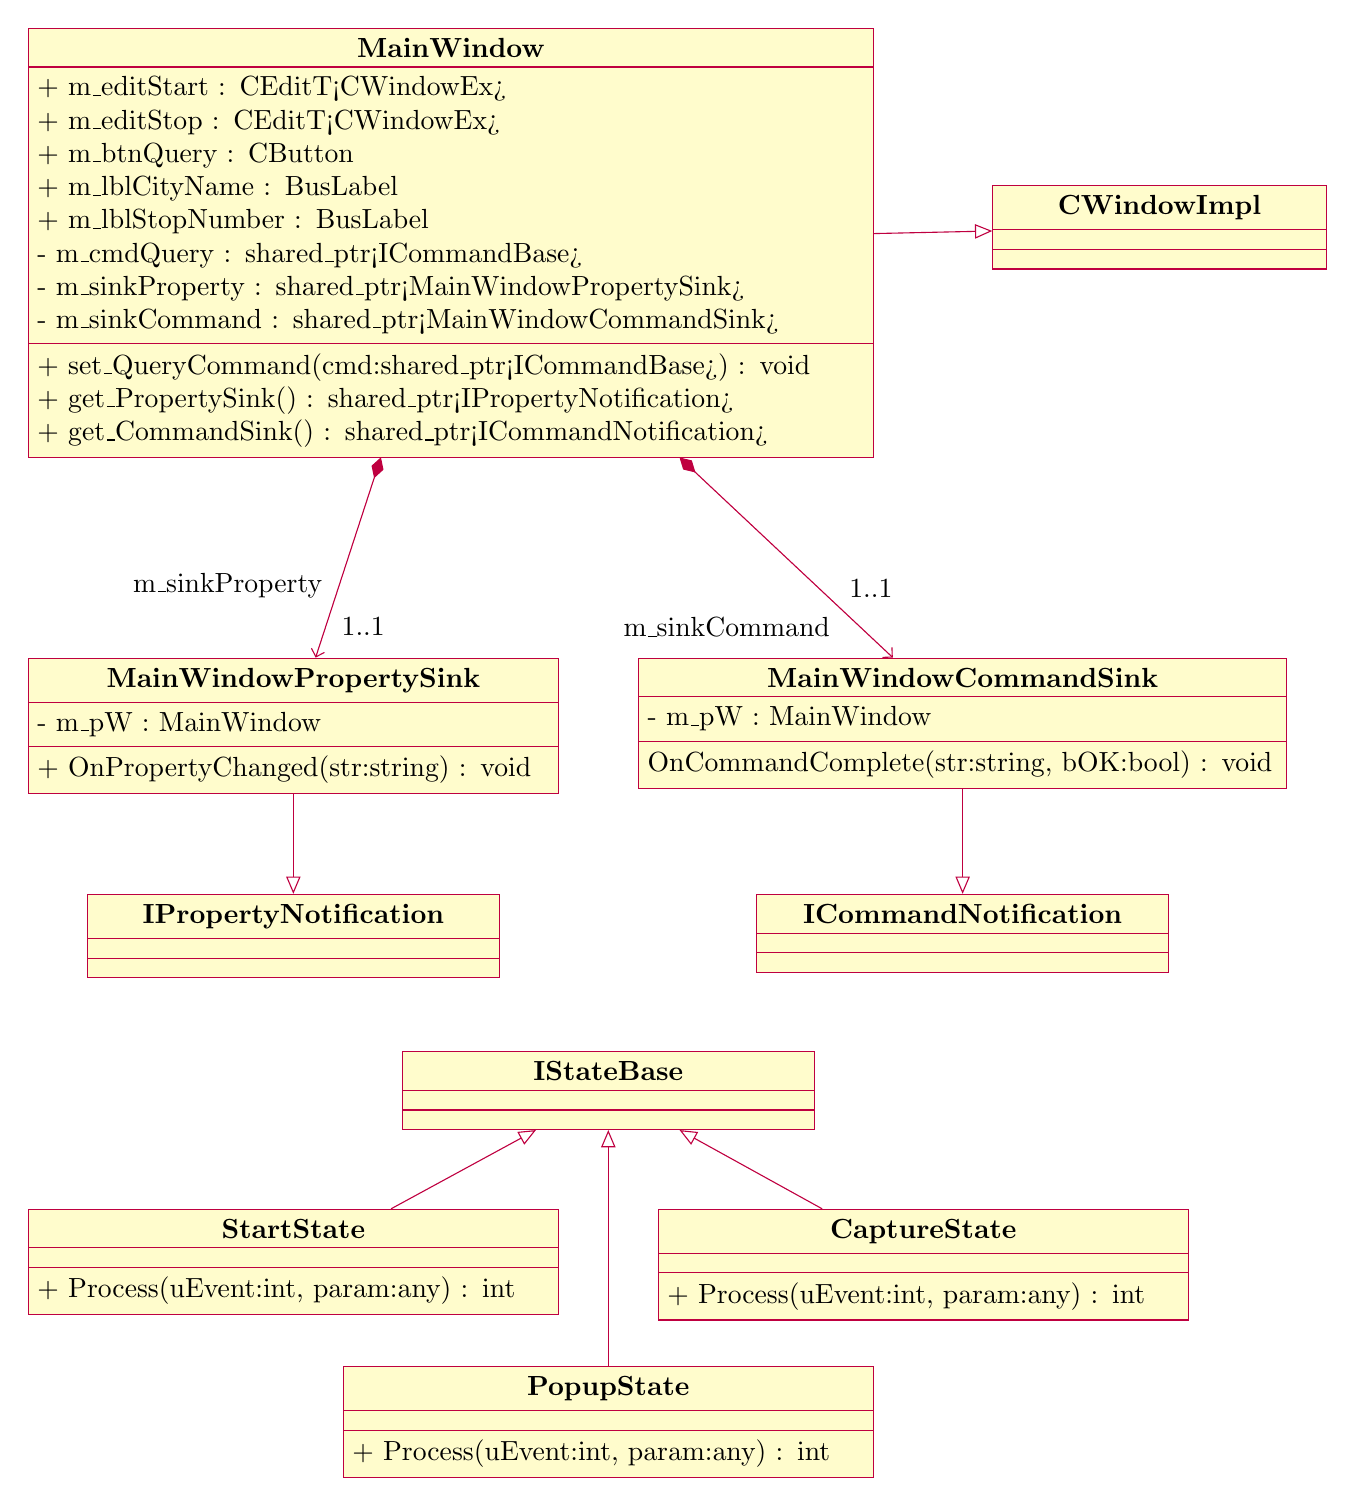
\begin{tikzpicture}
\begin{class}{IStateBase}{2,-13}\end{class}
\begin{class}[text width=6.5cm]{StartState}{-2,-15}
\inherit{IStateBase}
\operation{+ Process(uEvent:int, param:any) : int}
\end{class}
\begin{class}[text width=6.5cm]{PopupState}{2,-17}
\inherit{IStateBase}
\operation{+ Process(uEvent:int, param:any) : int}
\end{class}
\begin{class}[text width=6.5cm]{CaptureState}{6,-15}
\inherit{IStateBase}
\operation{+ Process(uEvent:int, param:any) : int}
\end{class}
\begin{class}[text width=4cm]{CWindowImpl}{9,-2}
\end{class}
\begin{class}[text width=10.5cm]{MainWindow}{0,0}
\inherit{CWindowImpl}
\attribute{+ m\_editStart : CEditT<CWindowEx>}
\attribute{+ m\_editStop : CEditT<CWindowEx>}
\attribute{+ m\_btnQuery : CButton}
\attribute{+ m\_lblCityName : BusLabel}
\attribute{+ m\_lblStopNumber : BusLabel}
\attribute{- m\_cmdQuery : shared\_ptr<ICommandBase>}
\attribute{- m\_sinkProperty : shared\_ptr<MainWindowPropertySink>}
\attribute{- m\_sinkCommand : shared\_ptr<MainWindowCommandSink>}
\operation{+ set\_QueryCommand(cmd:shared\_ptr<ICommandBase>) : void}
\operation{+ get\_PropertySink() : shared\_ptr<IPropertyNotification>}
\operation{+ get\_CommandSink() : shared\_ptr<ICommandNotification>}
\end{class}
\begin{class}{IPropertyNotification}{-2,-11}\end{class}
\begin{class}[text width=6.5cm]{MainWindowPropertySink}{-2,-8}
\inherit{IPropertyNotification}
\attribute{- m\_pW : MainWindow}
\operation{+ OnPropertyChanged(str:string) : void}
\end{class}
\begin{class}{ICommandNotification}{6.5,-11}\end{class}
\begin{class}[text width=8cm]{MainWindowCommandSink}{6.5,-8}
\inherit{ICommandNotification}
\attribute{- m\_pW : MainWindow}
\operation{OnCommandComplete(str:string, bOK:bool) : void}
\end{class}
\composition{MainWindow}{1..1}{m\_sinkProperty}{MainWindowPropertySink}
\composition{MainWindow}{1..1}{m\_sinkCommand}{MainWindowCommandSink}
\end{tikzpicture}
\newpage

\section{App Layer}
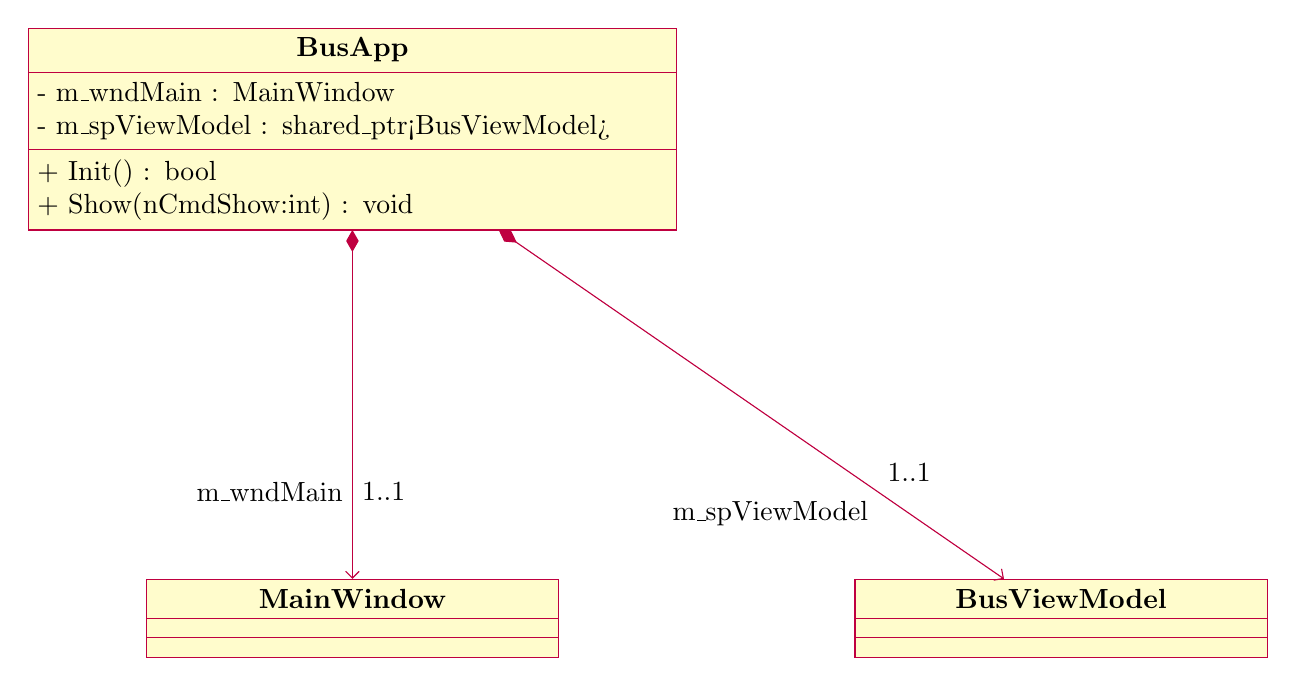
\begin{tikzpicture}
\begin{class}{MainWindow}{0,-7}\end{class}
\begin{class}{BusViewModel}{9,-7}\end{class}
\begin{class}[text width=8cm]{BusApp}{0,0}
\attribute{- m\_wndMain : MainWindow}
\attribute{- m\_spViewModel : shared\_ptr<BusViewModel>}
\operation{+ Init() : bool}
\operation{+ Show(nCmdShow:int) : void}
\end{class}
\composition{BusApp}{1..1}{m\_spViewModel}{BusViewModel}
\composition{BusApp}{1..1}{m\_wndMain}{MainWindow}
\end{tikzpicture}
\end{document}
